\section{Experiments and reproducibility}
\label{sec:experiments}

This repository is organized so that every paper figure is generated by an explicit script,
with parameters and deterministic metadata recorded at runtime.
We emphasize again: the experiments in this section are \emph{diagnostics}, not proofs.
Their role is to (i) validate that the tooling is numerically consistent with the accounting-style
quantities we discuss, and (ii) provide empirical evidence for (or against) the proposed
SBT-legality / anti-localization hinge.

\subsection{Manifest-driven figure generation (single source of truth)}

The canonical list of paper artifacts is the manifest
\nolinkurl{paper/figures_manifest.json}.
Each manifest entry records:
(i) the producing script, (ii) a deterministic seed, (iii) the expected output paths for a
\texttt{.png} and a companion \texttt{.npz}, and (iv) stdout markers used as a lightweight check.

To generate \emph{all} figures (including slow ones) into \texttt{python/artifacts/paper/}, run:
\begin{verbatim}
python/scripts/ns_paper_figures.py --include-slow --clean
\end{verbatim}
To generate only the fast subset (intended for CI and quick checks), run:
\begin{verbatim}
python/scripts/ns_paper_figures.py --clean
\end{verbatim}

\subsection{Determinism and metadata}

Each figure script prints a JSON configuration line of the form:
\texttt{FIGURE\_CONFIG: \{...\}},
including the seed and simulation parameters (grid size, timestep, forcing parameters, thresholds).
Each figure also writes a companion \texttt{.npz} containing the plotted arrays and key scalars.
This enables two kinds of reproducibility:
\begin{itemize}
\item \textbf{Re-plot reproducibility:} the \texttt{.npz} contains all data needed to recreate the plot.
\item \textbf{Run determinism checks:} for the fast set, the generator supports
\texttt{--verify-determinism}, which re-runs the figure scripts and checks that the resulting
\texttt{.npz} hashes match.
\end{itemize}
In other words, the paper artifacts are treated like build products with a testable provenance chain.

\paragraph{Determinism scope.}
Our determinism checks verify byte-identical \texttt{.npz} outputs when rerunning in a fixed
software environment (same code, dependencies, and backend behavior). We do not claim bitwise
identity across arbitrary BLAS/FFT backends or thread schedules; for cross-platform reruns we
recommend pinning threads (e.g.\ \texttt{OMP\_NUM\_THREADS=1}, \texttt{MKL\_NUM\_THREADS=1})
and using tolerance-based numeric comparisons where appropriate.

\paragraph{Fast vs.\ slow figures.}
The manifest classifies figures as fast/slow/optional. Fast figures are intended for CI-style
checks, while slow figures are diagnostic enrichments and are not required for any mechanized claim.

\subsection{Main diagnostic figures (evidence, not proofs)}

We include a small set of representative figures in the main text.
The full index of paper artifacts (script $\leftrightarrow$ figure mapping) is maintained in
\texttt{docs/fluids/blowup/figures.md} and in the manifest.

\paragraph{Channel count (effective rank) by shell.}
This diagnostic estimates a minimal channel count $m_{95}$ capturing $95\%$ of shell variance
under a windowed PCA/SVD procedure. It is one empirical proxy for the ``finite channel'' premise
used in the anti-localization lemma template.

\paragraph{Interpreting pooled vs.\ windowed effective ranks.}
We report both windowed ranks (computed per time window) and pooled ranks (computed after pooling
snapshots across time and seeds). A pooled rank can exceed typical windowed ranks if the dominant
channel rotates over time: each window may be effectively one-dimensional, while the pooled dataset
spans a small subspace of dimension $>1$. We treat these as diagnostics of low-channel structure,
not as proof of a fixed global rank.

\begin{figure}[t]
  \centering
  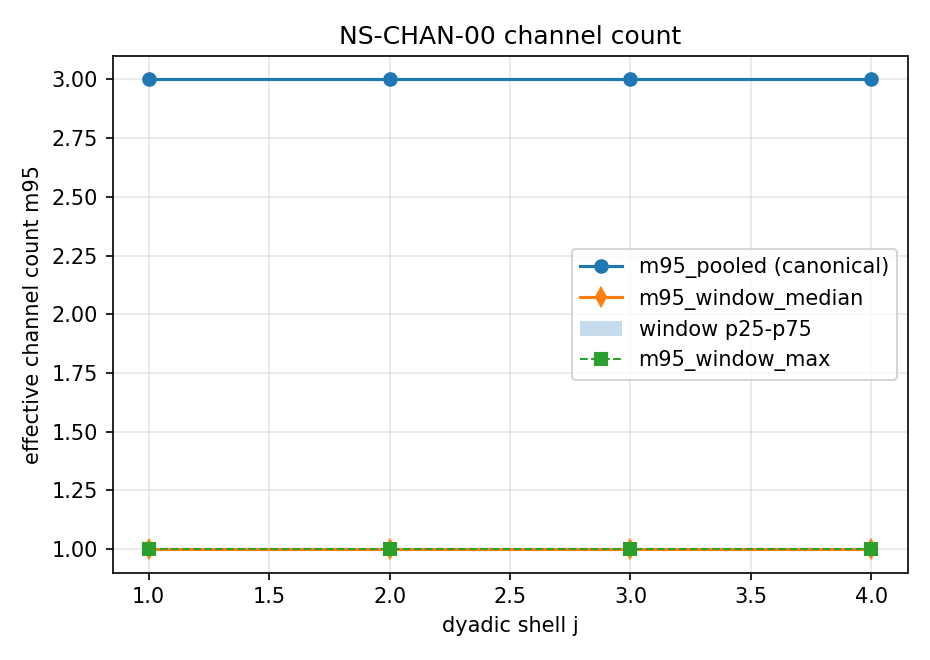
\includegraphics[width=0.92\linewidth]{../python/artifacts/paper/ns_channel_count.png}
  \caption{\textbf{Empirical channel count by shell.}
  We estimate an effective rank $m_{95}(j)$ capturing 95\% of variance from shell snapshots
  (pooled across seeds and windows; see script for details).
  This is diagnostic evidence relevant to finite-channel / sectorization narratives.}
  \label{fig:channel-count}
\end{figure}

\paragraph{Delocalization of learned channels.}
Given the channel decomposition used in Fig.~\ref{fig:channel-count}, we measure a delocalization proxy
for the extracted channel shapes and report an induced $\hat\eta_j$ consistent with
\eqref{eq:antiloc}--\eqref{eq:finite-channel-antiloc} (up to discretization and estimator choices).

\begin{figure}[t]
  \centering
  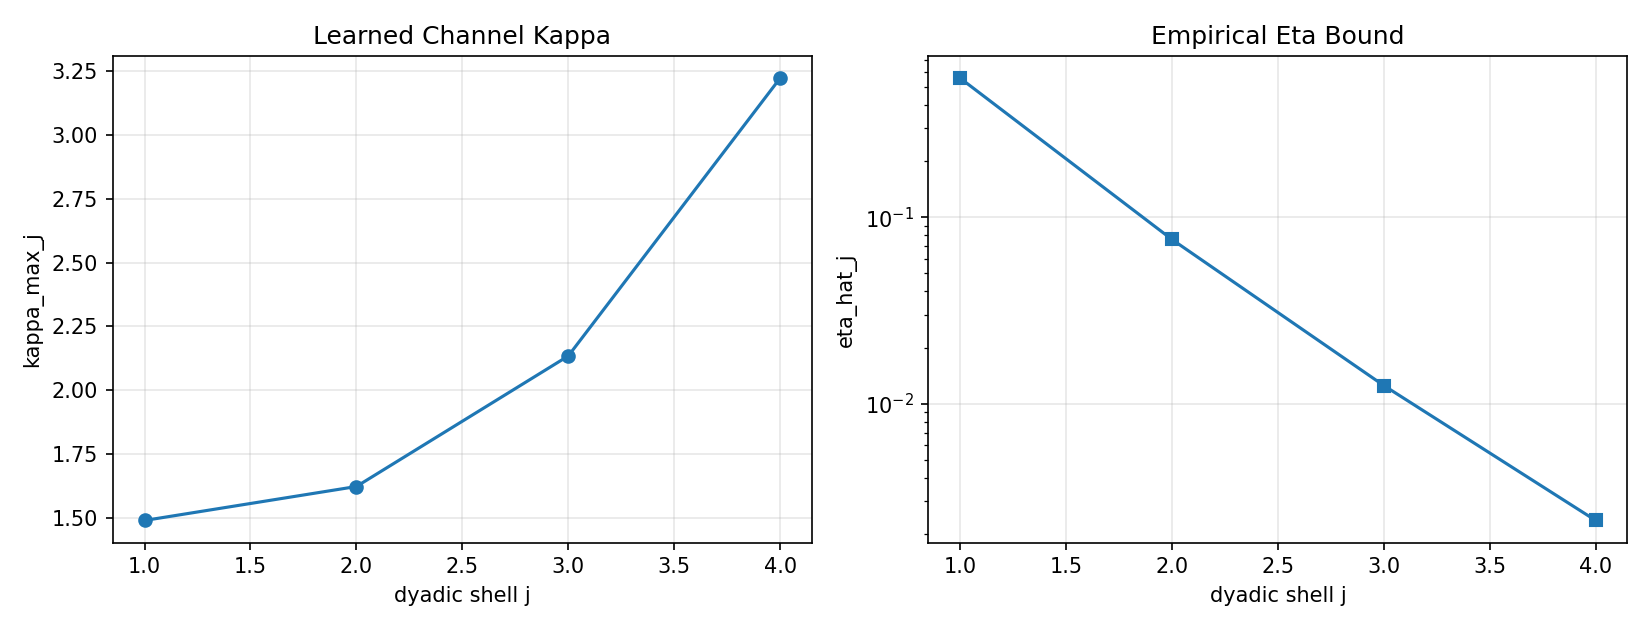
\includegraphics[width=0.92\linewidth]{../python/artifacts/paper/ns_channel_delocalization.png}
  \caption{\textbf{Empirical channel delocalization and induced anti-localization bound.}
  For each shell $j$, we evaluate a local mass functional on the learned channel shapes and report
  a worst-case delocalization proxy $\kappa$ and an induced $\hat\eta_j$.
  This is diagnostic-only evidence toward the anti-localization hinge.}
  \label{fig:channel-delocalization}
\end{figure}

\paragraph{Anti-localization sweep (SBT-legality evidence).}
We run a small sweep of short forced simulations and compute worst-case anti-localization metrics
over time windows (see Section~\ref{sec:spt-legal} for definitions). This is intended to answer:
``in tested regimes, do shell fields tend to avoid wavepacket-like localization?''

\begin{figure}[t]
  \centering
  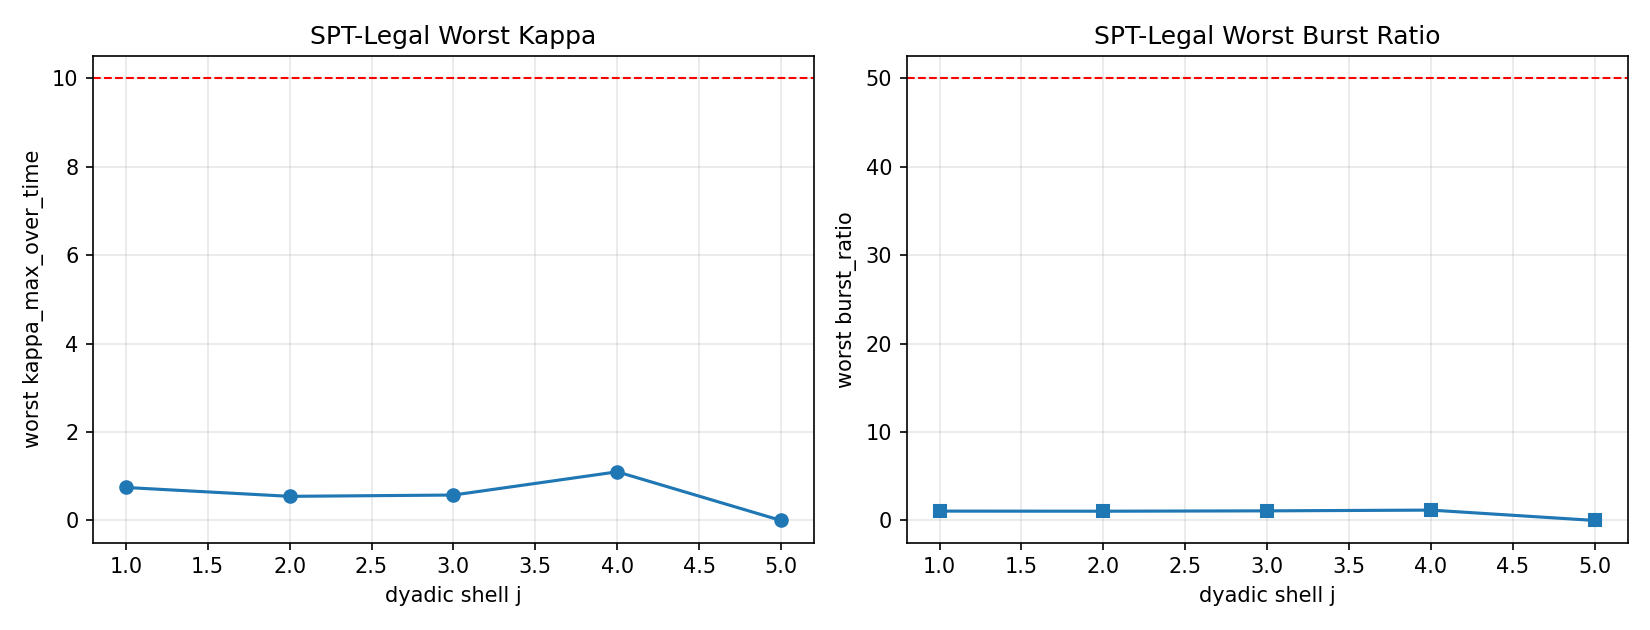
\includegraphics[width=0.92\linewidth]{../python/artifacts/paper/ns_spt_legal_sweep.png}
  \caption{\textbf{Anti-localization sweep (diagnostic).}
  Worst-case $\kappa_j$-style concentration factors over a small parameter/seed sweep.
  This supports plausibility of an anti-localization restriction in the tested window, but is not
  a worst-case theorem for Navier--Stokes.}
  \label{fig:spt-legal-sweep}
\end{figure}

\paragraph{LEGAL vs.\ ILLEGAL initial data (certificate nontriviality).}
Figure~\ref{fig:spt-illegal-vs-legal} (in Section~\ref{sec:spt-legal}) demonstrates that the
certificate is not vacuous: an intentionally localized shell construction fails immediately.

\paragraph{Toy Zeno gallery (intuition anchor).}
Finally, we include a purely mathematical toy gallery showing why the No-Zeno engine requires
both a work quantization and a divergence condition: with fast-growing capacity (or vanishing work),
Zeno can occur even when other bookkeeping looks benign.

\begin{figure}[t]
  \centering
  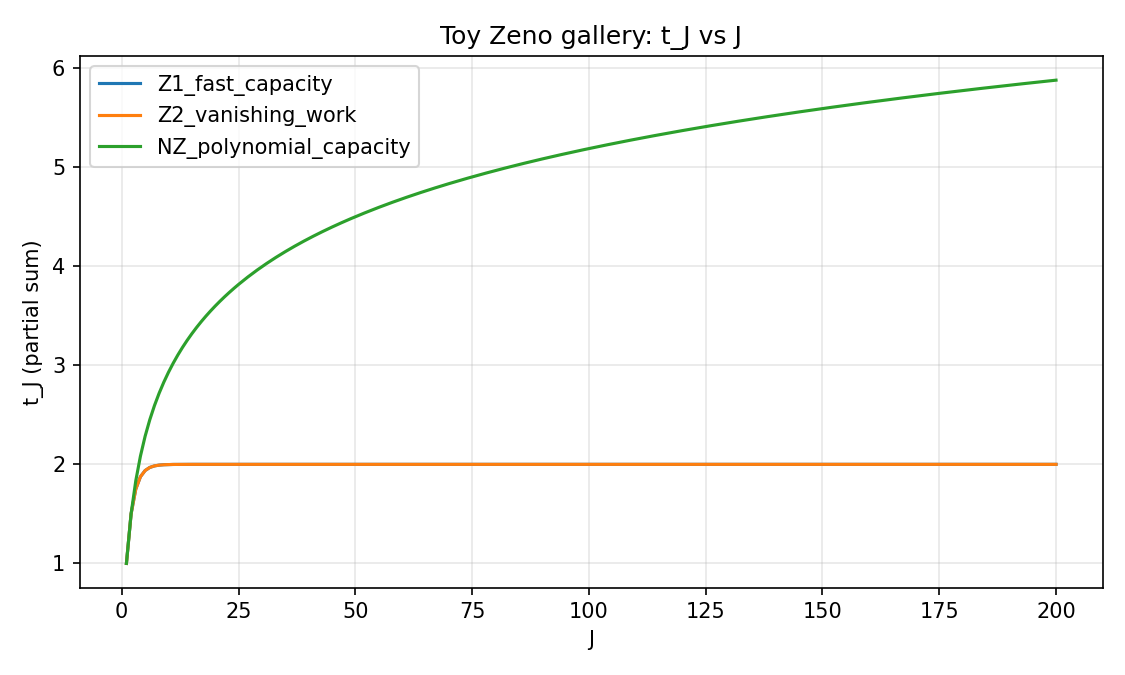
\includegraphics[width=0.92\linewidth]{../python/artifacts/paper/nsbu12_toy_zeno_gallery.png}
  \caption{\textbf{Toy Zeno gallery.}
  Three explicit sequences illustrate: (i) Zeno via fast-growing capacity (DIV fails),
  (ii) Zeno via vanishing work quantum (WORK fails), and (iii) a No-Zeno control with polynomial capacity.
  This figure is purely mathematical and serves as an intuition anchor for the mechanized No-Zeno logic.}
  \label{fig:toy-zeno}
\end{figure}
